\documentclass[11pt]{standalone}

\usepackage{helvet}
\usepackage{units}
\usepackage{textcomp}

\usepackage{ifthen}
\usepackage{tikz} 
\usetikzlibrary{shapes.misc}
\usetikzlibrary{arrows,arrows.meta}
\usetikzlibrary{calc,intersections, patterns, math}
\usetikzlibrary{decorations.pathmorphing}
\usetikzlibrary{shapes.geometric}

\definecolor{pfeil}{RGB}{168,167,167}
\definecolor{petrol}{RGB}{0, 118, 136}
\definecolor{darkgoldenrod}{RGB}{184, 134, 11}
\colorlet{petrol-lighter}{petrol!40}
\colorlet{darkgoldenrod-lighter}{darkgoldenrod!40}

\newcommand{\polygon}[3]{ 
    % #1 = position
    % #2 = anzahl ecken
    % #3 = farbe 
    \pgfmathsetmacro{\MyRand}{3.6*random(0,100)}
    \node[#3, fill,regular polygon,draw,
	regular polygon sides = #2, rotate=\MyRand] at (#1) {\phantom{.}};
}

\begin{document}

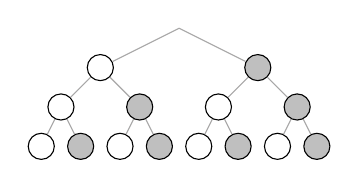
\begin{tikzpicture}[pfeil,
    circ/.style={draw=black,circle},
    grow=down,
    level 1/.style={sibling distance=2cm},
    level 2/.style={sibling distance=1cm},
    level 3/.style={sibling distance=0.5cm},
    level distance=0.5cm]
    \node [coordinate] at(0,0) {}
    child {
        node[circ] {}
        child { node[circ] {}
            child { node[circ] {}
                edge from parent}
            child { node[circ,fill=lightgray] {}
                edge from parent}
            edge from parent
        }
        child { node[circ,fill=lightgray] {}
            child { node[circ] {}
                edge from parent}
            child { node[circ,fill=lightgray] {}
                edge from parent}
            edge from parent
        }
        edge from parent
    }
    child {
        node[circ,fill=lightgray] {}
        child { node[circ] {}
            child { node[circ] {}
                edge from parent}
            child { node[circ,fill=lightgray] {}
                edge from parent}
            edge from parent 
        }
        child { node[circ,fill=lightgray] {}
            child { node[circ] {}
                edge from parent}
            child { node[circ,fill=lightgray] {}
                edge from parent}
            edge from parent
        }
        edge from parent
    };
   

    




\end{tikzpicture}




\end{document}
